% Created 2018-04-24 Tue 09:48
% Intended LaTeX compiler: pdflatex
\documentclass[10pt]{beamer}
\usepackage[utf8]{inputenc}
\usepackage[T1]{fontenc}
\usepackage{graphicx}
\usepackage{grffile}
\usepackage{longtable}
\usepackage{wrapfig}
\usepackage{rotating}
\usepackage[normalem]{ulem}
\usepackage{amsmath}
\usepackage{textcomp}
\usepackage{amssymb}
\usepackage{capt-of}
\usepackage{hyperref}
\usetheme{Boadilla}
\author{ECON 499: Growth and Development}
\date{Spring 2018}
\title{Human Capital}
\usecolortheme{seagull}
\usefonttheme[onlylarge]{structurebold}
\usefonttheme[onlymath]{serif}
\setbeamerfont*{frametitle}{size=\normalsize,series=\bfseries}
\setbeamertemplate{navigation symbols}{}
\setbeamertemplate{itemize item}[triangle]
\setbeamertemplate{footline}{}
\setbeamertemplate{enumerate items}[default]
\hypersetup{
 pdfauthor={ECON 499: Growth and Development},
 pdftitle={Human Capital},
 pdfkeywords={},
 pdfsubject={},
 pdfcreator={Emacs 25.2.2 (Org mode 9.1.6)}, 
 pdflang={English}}
\begin{document}

\maketitle

\begin{frame}[label={sec:org2b5530b}]{}
\alert{Growth in the Solow model}
\begin{itemize}
\item Output (income) is created by combining labor and capital
\item Capital accumulation increases income (workers become more productive)
\item As workers save (invest) more, the have more capital to utilize in the future
\item Solow model assumes labor is homogeneous, same across countries
\item Given the same capital, does the average worker in North Korea have the same productivity as the average worker in Germany?
\end{itemize}
\end{frame}

\begin{frame}[label={sec:orgbc1c7b6}]{}
\alert{Human capital}
\begin{itemize}
\item \emph{Human capital} is a set of individual characteristics that affect the productivity of workers
\item Not an exhaustive set (innate ability is \emph{not} considered human capital)
\item Workers with high human capital are more productive
\item Human capital can be changed, either through behavior or policy
\item Examples: Health, education
\end{itemize}
\end{frame}

\begin{frame}[label={sec:orgad59ee4}]{}
\alert{Properties of human capital}

Similar to physical capital, human capital is:
\begin{enumerate}
\item Productive
\item Produced
\item Earns a return (higher wages)
\item Depreciating
\end{enumerate}
\end{frame}

\begin{frame}[label={sec:orgb62c89d}]{}
\alert{Health}
\begin{itemize}
\item Healthy people can work longer, harder than unhealthy people
\item Health human capital can be difficult to measure, must rely on "proxy" variables
\item Height and available calories are commonly used proxies
\item In 1855, 2/3 of Dutch men were shorter than 5'6'', less than 2\% today
\end{itemize}
\end{frame}

\begin{frame}[label={sec:org0158144}]{}
\begin{center}
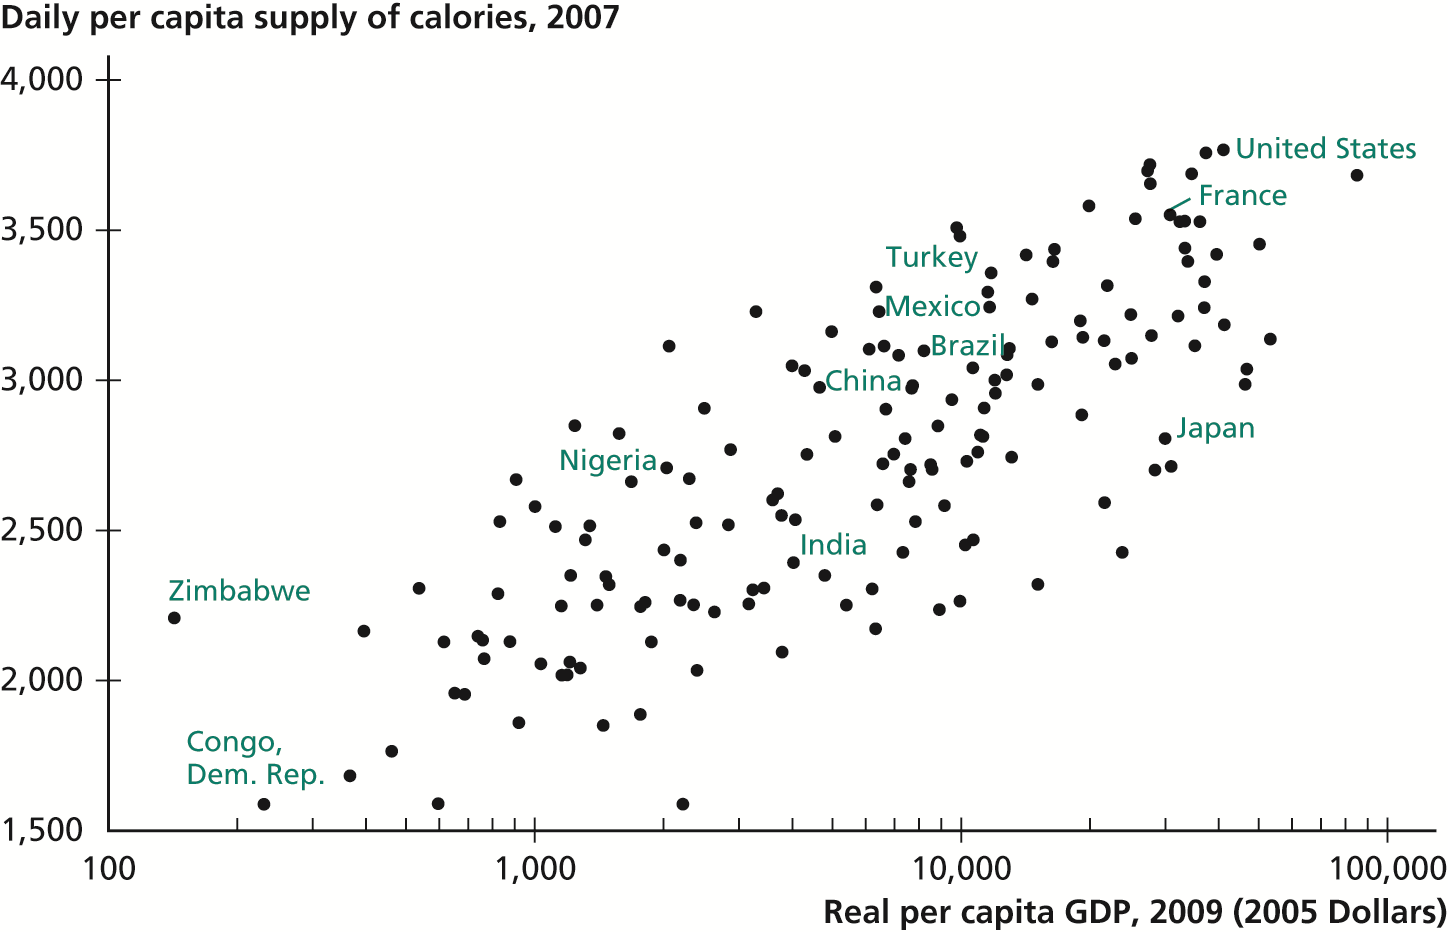
\includegraphics[width=.75\textwidth]{./img/6.1.png}
\end{center}
\end{frame}

\begin{frame}[label={sec:orga4c21fc}]{}
\alert{Malnourishment divide}
\begin{itemize}
\item Very few people are malnourished in the developed world
\item Fogel (1997): 20\% of adults in 1780 Britain did not have enough calories to provide energy to work 1 hour per day, contributed to 0.33\% additional growth per year
\item Malnourishment still a chronic problem in developing world
\item In addition to calories, many lack essential vitamins and minerals, affects wages and ability to work, health outcomes
\end{itemize}
\end{frame}

\begin{frame}[label={sec:org1004679}]{}
\begin{center}
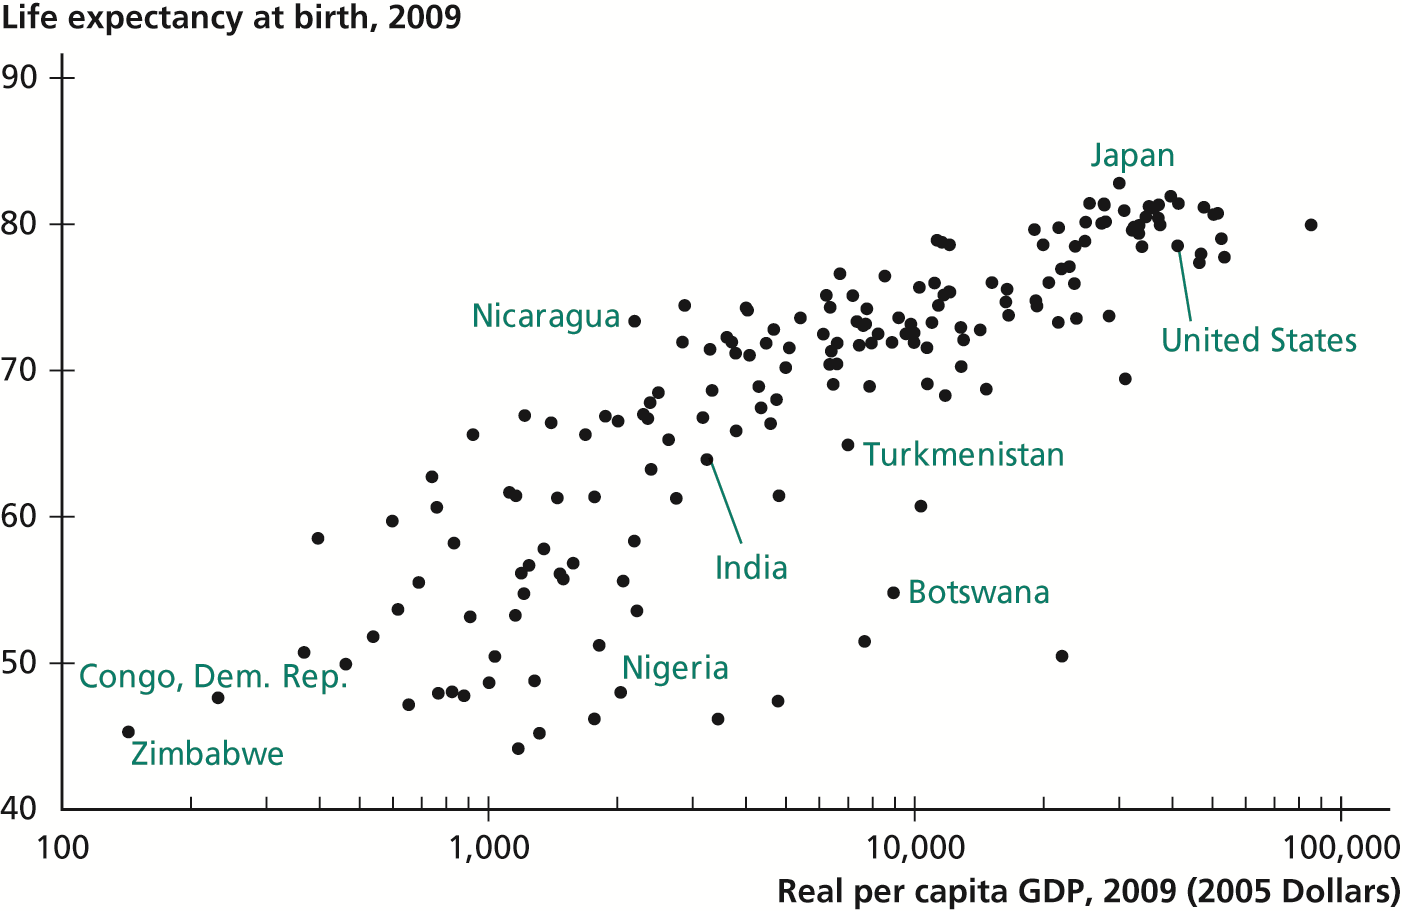
\includegraphics[width=.75\textwidth]{./img/6.2.png}
\end{center}
\end{frame}

\begin{frame}[label={sec:org5c37440}]{}
\alert{Simultaneity of health and income}

Health and income are \emph{simultaneously determined}
\begin{itemize}
\item Health can affect ability to earn income
\item Income allows people to buy more food, health care, etc
\item Creates multiplier effects, feedback between health and income
\item Creates difficulty in measuring relative importance of health vs income
\end{itemize}
\end{frame}

\begin{frame}[label={sec:orgb455094}]{}
\alert{Example: Malaria debate}

Jeffrey Sachs:
\begin{itemize}
\item Countries that have eliminated malaria have grown much more rapidly than countries that have high malaria rates
\item Malaria alone is responsible for a substantial portion of cross-country differences in growth and income
\item Micro evidence suggests that eliminating malaria can have large effects on human capital acquisition, productivity
\end{itemize}

Acemoglu, Johnson, Robinson:
\begin{itemize}
\item Countries differ in their \emph{ability} to combat malaria
\item Countries that are able to eliminate malaria have strong institutions, care about public health
\item Good institutions are responsible for growth and income, malaria reductions are a side effect
\end{itemize}
\end{frame}


\begin{frame}[label={sec:orga963f28}]{}
\alert{Education}
\begin{itemize}
\item Obvious relationship between education and productivity, wages
\item \emph{Return to schooling}: income derived from an additional year of school
\item Return is higher for early schooling (reading and writing marginally more valuable than learning how to solve the Solow model)
\item Omitted variable bias?
\end{itemize}
\end{frame}

\begin{frame}[label={sec:org984a7ce}]{}
\begin{center}
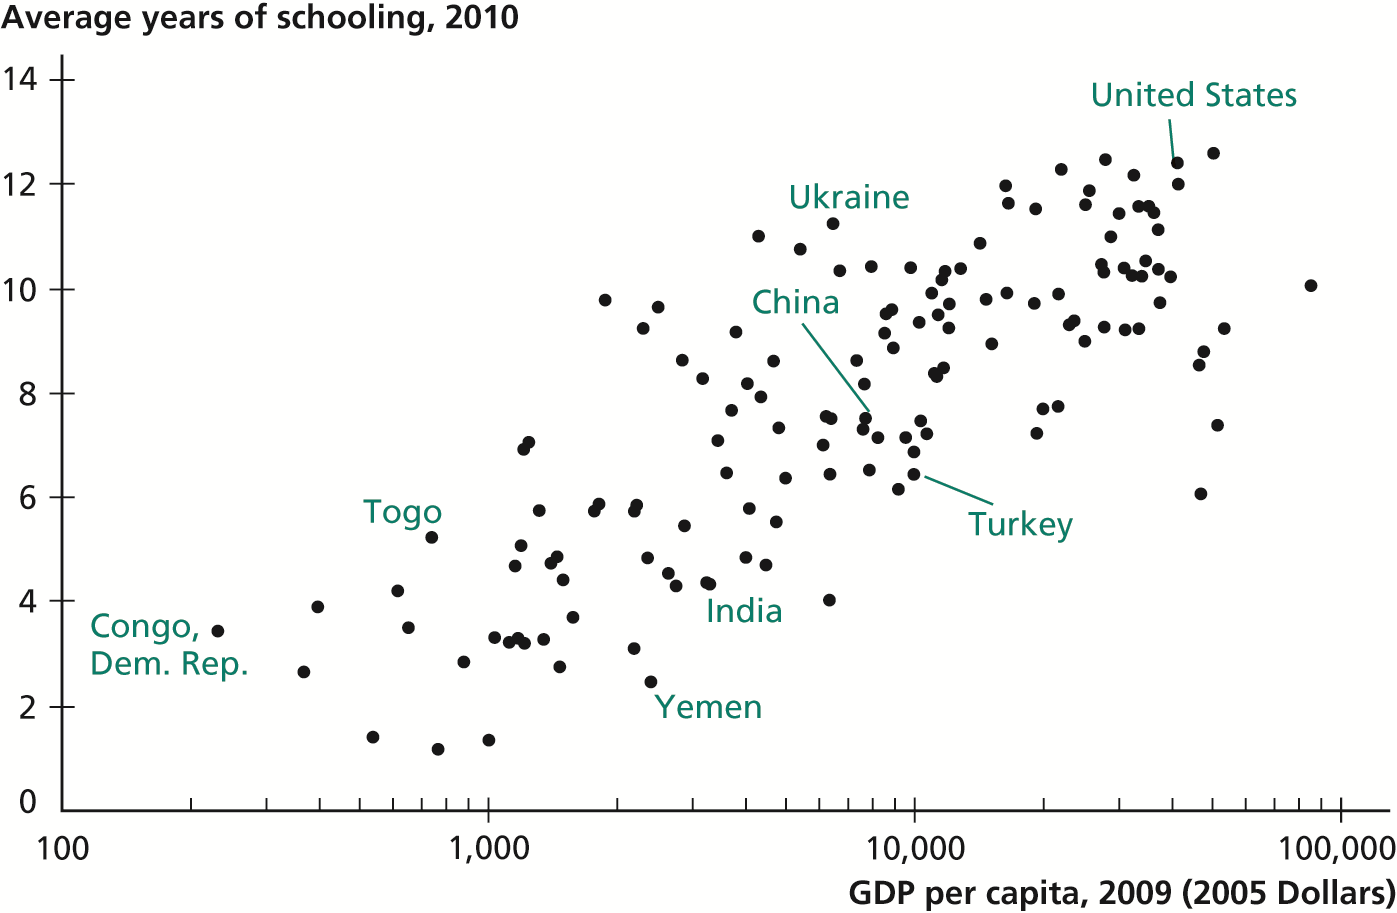
\includegraphics[width=.75\textwidth]{./img/6.11.png}
\end{center}
\end{frame}

\begin{frame}[label={sec:orgd917e50}]{}
\begin{center}
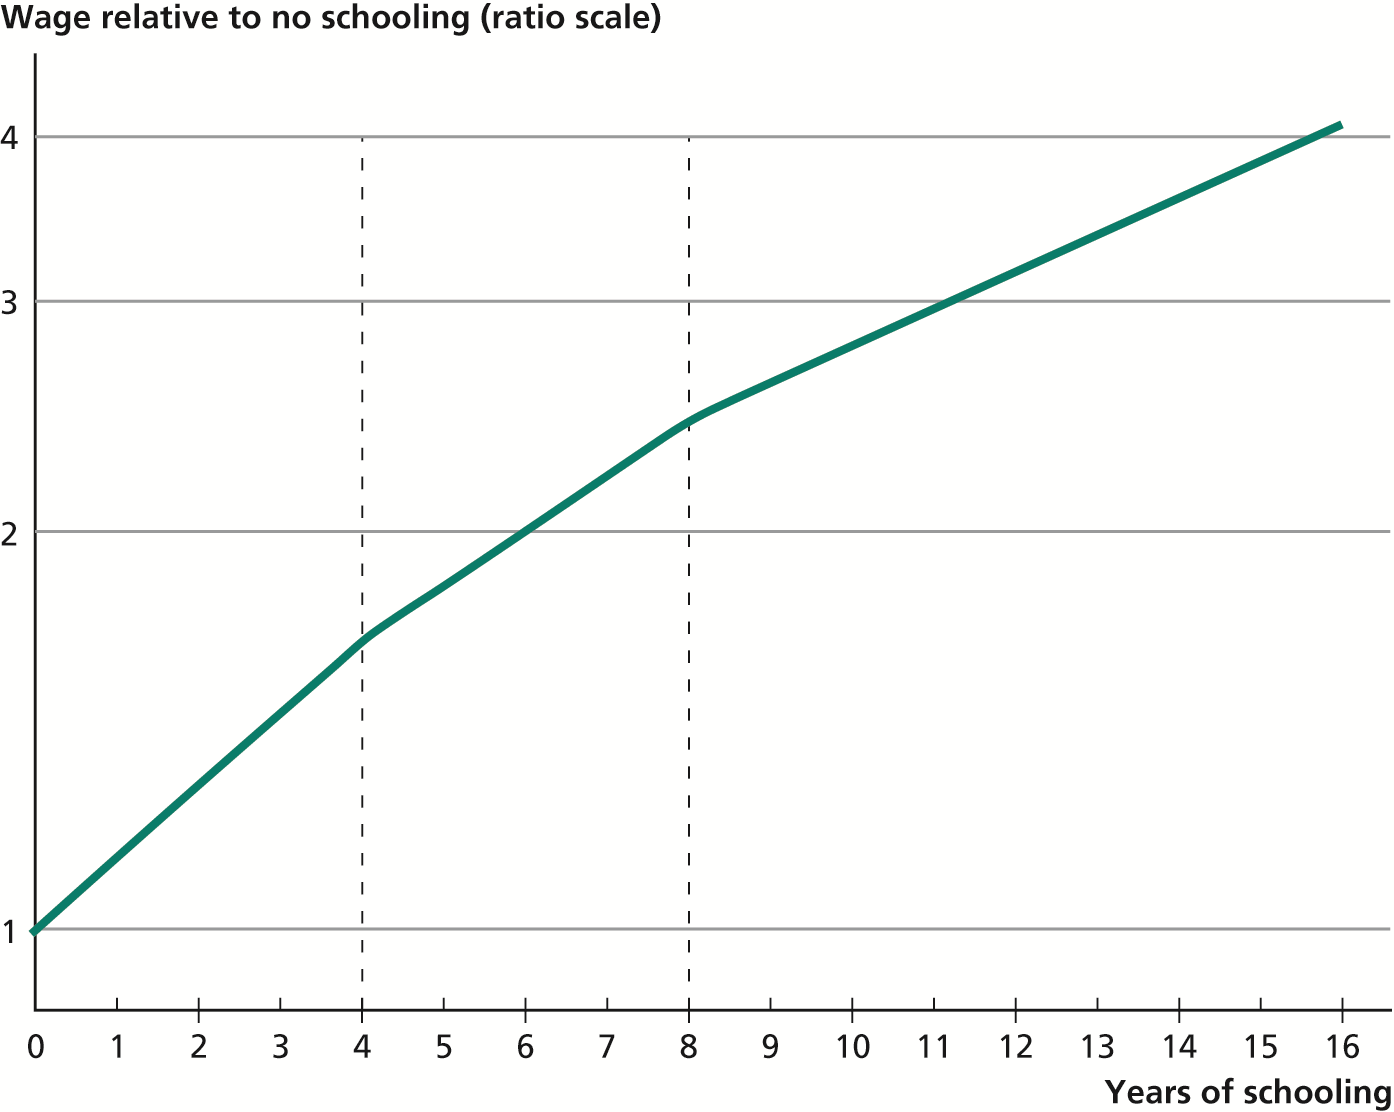
\includegraphics[width=.75\textwidth]{./img/6.6.png}
\end{center}
\end{frame}

\begin{frame}[label={sec:org9d63228}]{}
\alert{Human capital share of wages}
\begin{itemize}
\item How much of national income rewards human capital?
\item Alternatively, how large are the returns to education? How much cross-country difference can it explain?
\item Using returns to wages and national education levels, we can divide amount of income going to "raw labor" and amount going to human capital
\end{itemize}
\end{frame}

\begin{frame}[label={sec:orgbacc8a7}]{}
\begin{center}

\includegraphics[width=.75\textwidth]{./img/tab6.2.png}
\end{center}
\end{frame}

\begin{frame}[label={sec:org74d9a1e}]{Share of Human Capital in Wages in Developing Countries}
\begin{center}
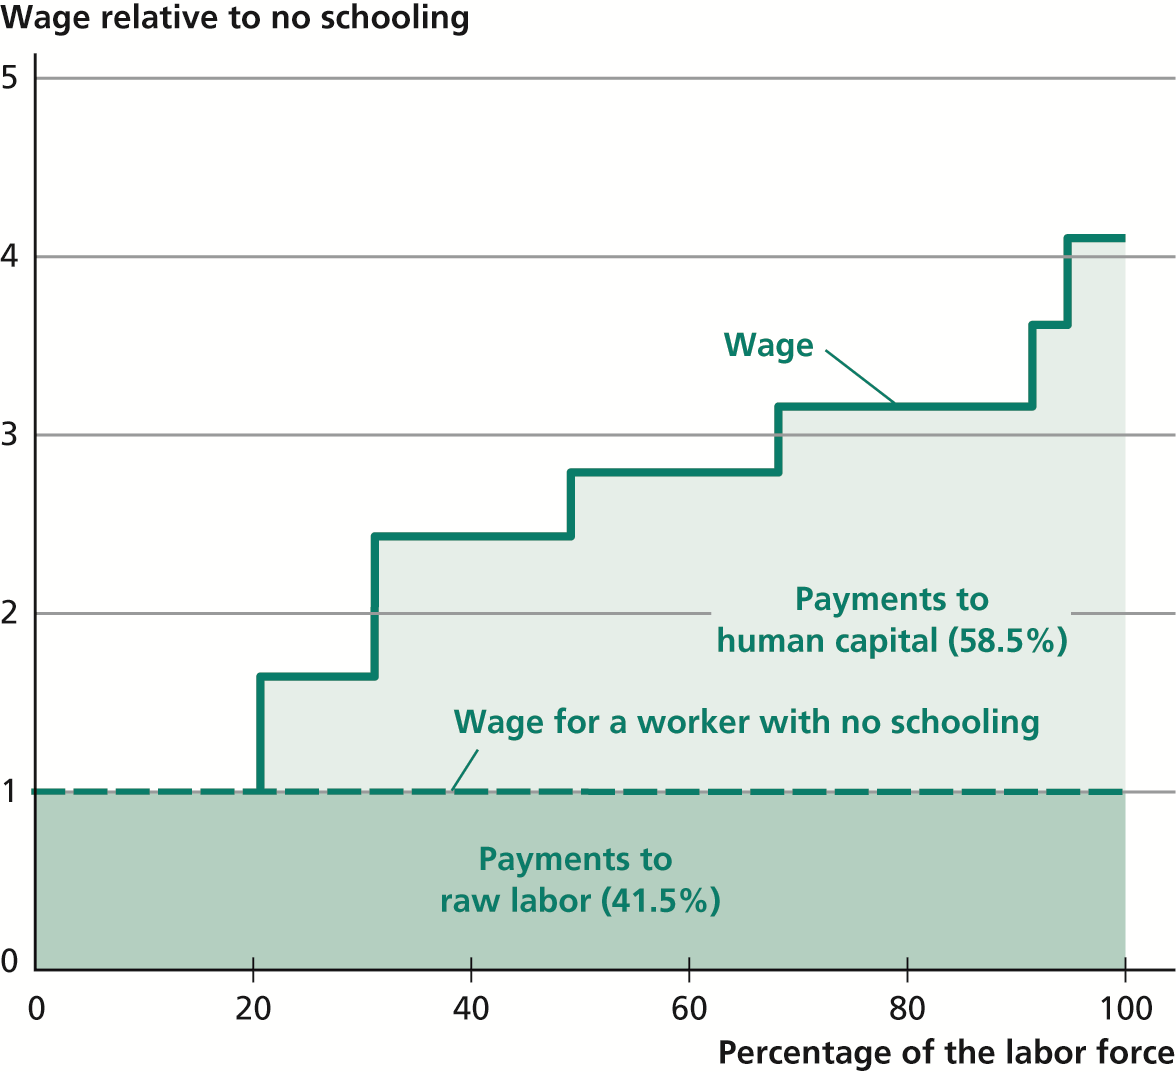
\includegraphics[width=.75\textwidth]{./img/6.9.png}
\end{center}
\end{frame}

\begin{frame}[label={sec:orge53b139}]{Share of Human Capital in Wages in Advanced Countries}
\begin{center}
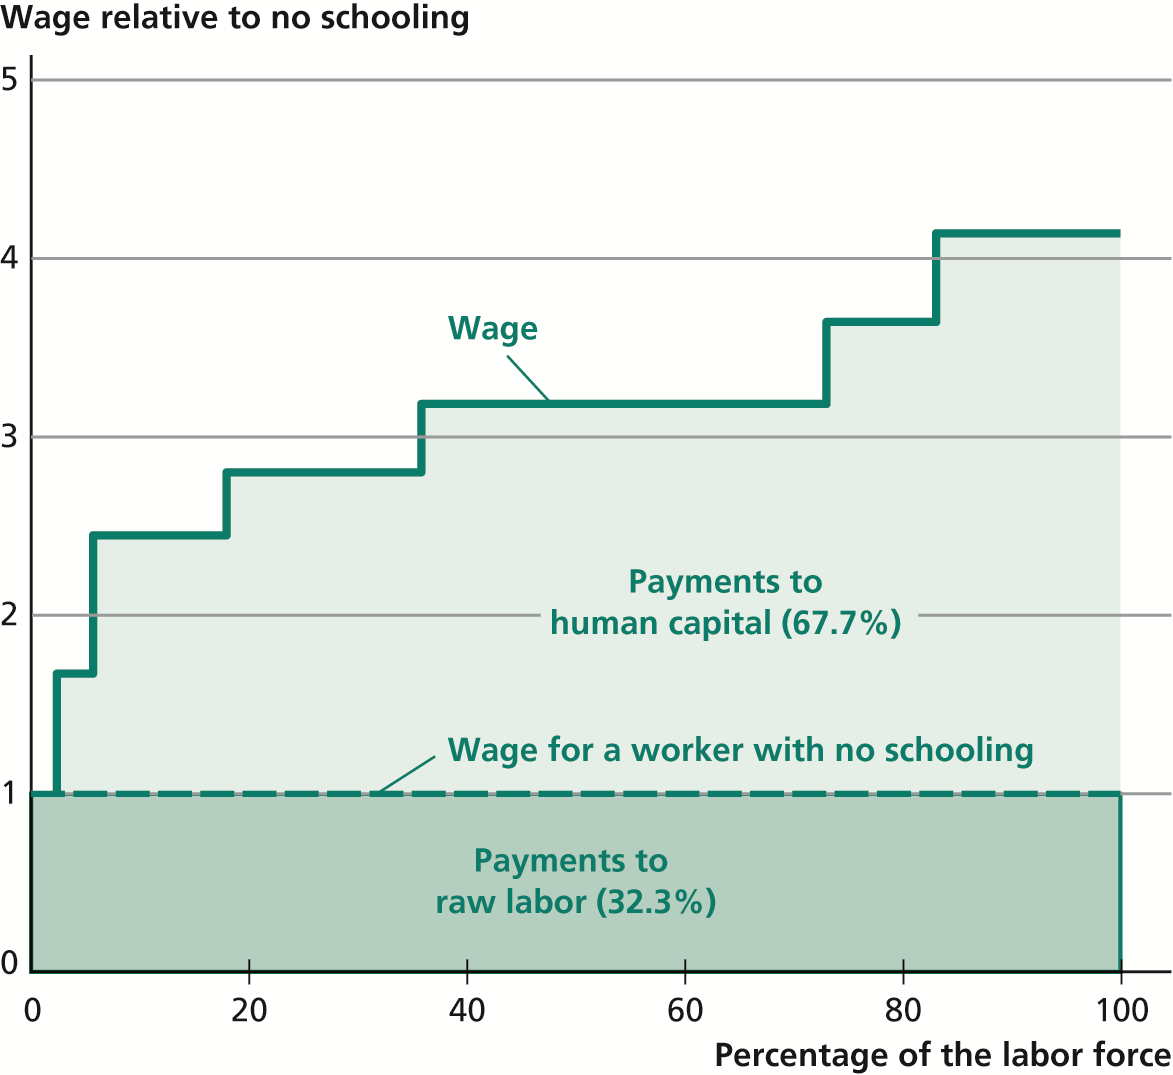
\includegraphics[width=.75\textwidth]{./img/6.10.png}
\end{center}
\end{frame}

\begin{frame}[label={sec:orgfff7292}]{}
\begin{center}
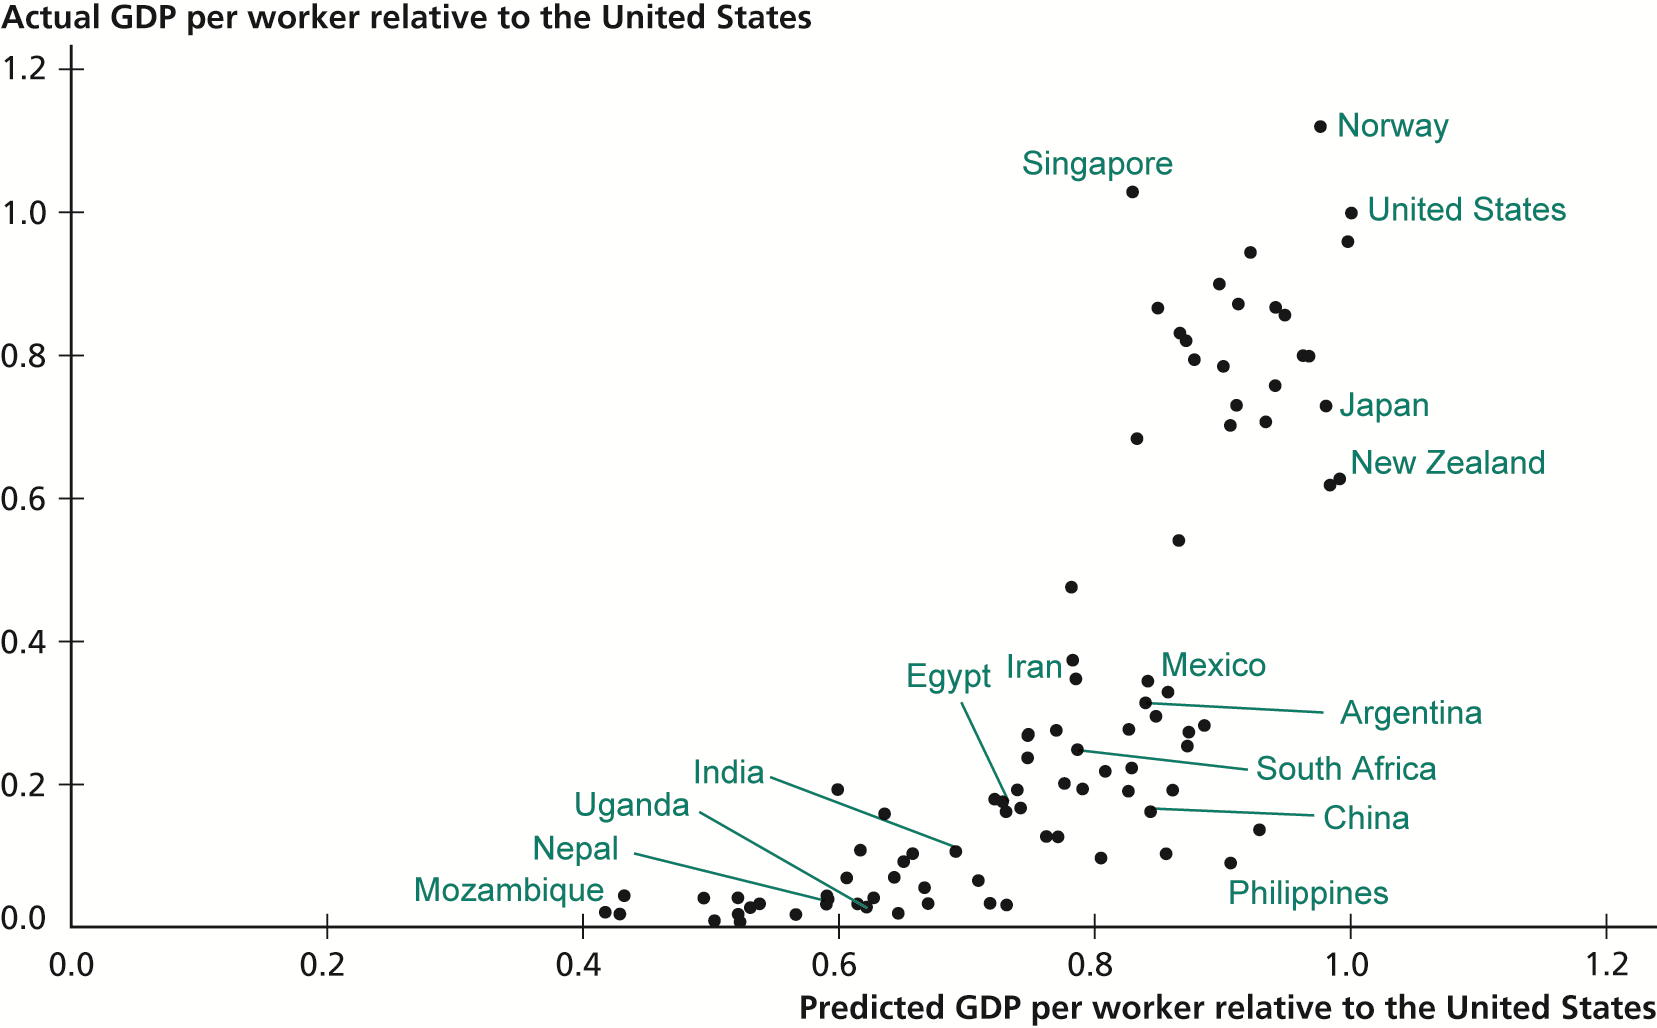
\includegraphics[width=.75\textwidth]{./img/6.12.png}
\end{center}
\end{frame}

\begin{frame}[label={sec:orgd2d5eec}]{}
\alert{Education in the Solow model}
\begin{itemize}
\item Cross-country differences in education explain much (but not all) of the difference in income
\item Model performs better for developed countries than developing countries
\item Developing countries are poorer than they "should" be given educational differences
\end{itemize}
\end{frame}

\begin{frame}[label={sec:org1498a74}]{}
\alert{Quantity vs quality}
\begin{itemize}
\item Years of schooling might be a bad measure of human capital attainment
\item 12 years in Sweden is different than 12 years in Mozambique
\item Teachers in developing world often have less training, fewer textbooks and other resources, worse attendance (students and teachers)
\end{itemize}
\end{frame}

\begin{frame}[label={sec:org6401cbb}]{}
\begin{center}
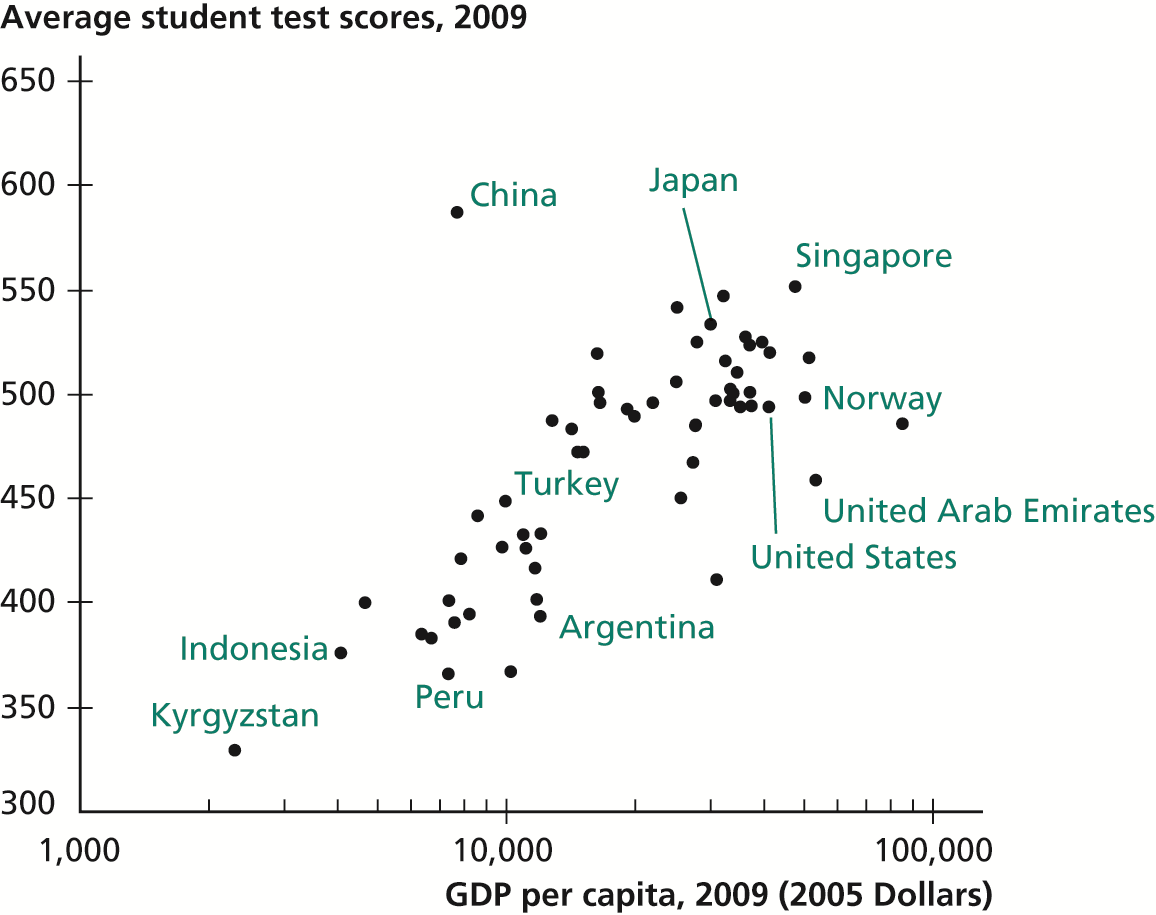
\includegraphics[width=.75\textwidth]{./img/6.13.png}
\end{center}
\end{frame}

\begin{frame}[label={sec:org293b9d1}]{}
\alert{Externalities}
\begin{itemize}
\item People invest in human capital and get a return in the form of higher wages
\item Investing in human capital may impact \alert{other} people as well (externality)
\item Educated workers more likely to adopt technology, other workers can then use that technology
\item Higher educated teachers can improve education of next generation
\item Educated workers may innovate, accumulate capital
\item Socially optimal education levels may be higher than levels chosen by fully rational people
\end{itemize}
\end{frame}
\end{document}